\section{Experimental Evaluation} \label{sec:experiments}

This section presents the research questions and the experiments that we conducted and analysed to to validate our approximate distributed monitoring approach.

\subsection{Research Questions}

We seek answers to the following research questions (RQs):

\begin{resq}[What is the tradeoff between the efficiency and the accuracy of approximate distributed monitors?]
The  approximate distributed monitoring comes with a price in terms of the loss of accuracy. We want to understand what is the tradeoff between the potential speed-ups that an approximate distributed monitor can potentially achieve when compared to its exact counterpart and the consequent loss in accuracy due to the approximations. We would also like to identify the classes of signals and properties for which this tradeoff is effective. 
\end{resq}

\begin{resq}[Can the combination of approximate and exact distributed monitors increase efficiency while preserving accuracy?]
We are interested in evaluating whether a smart combined use of approximate and exact distributed monitors can still bring improvements in monitoring efficiency while guaranteeing the accuracy of the monitoring verdicts. 
\end{resq}

\subsection{Experimental Setup}

\subsubsection{Distributed Monitors} \label{sec:testGeneration}
In our study, we compare our approximate distributed monitoring (ADM) approach to a an exact distributed monitoring approach. For the exact monitoring, we take a variant of the distributed monitoring procedure from~\cite{MomtazAB23} that allows to evaluate STL specifications over distributed traces using SMT-solving. Originally, that procedure assumes that input signals are polynomial continuous functions. We adapt the SMT-based approach to consider input signals as piecewise-constant signals to make a consistent comparison with ADM. We note that the passage from the polynomial continuous to piecewise-constant input signals reduces the efficiency of the SMT-based monitors. We also observe that the SMT-based monitors from~\cite{MomtazAB23} can split the input trace into multiple segments and evaluate the specification incrementally, segment-by-segment, allowing early termination of the monitor in some cases. Since the focus of this paper is purely on the offline monitoring, we also use the exact monitors without their incremental mode. We use the abbreviation EDM to denote the variant of the exact SMT-based distributed monitors used in this study.


\subsubsection{Experimental Subjects}
To answer our research questions, we also use a \emph{random generator} (RG) of distributed traces, in which we can control the trace duration $d$ (in terms of the number of events) and the bound on the clock skew $\varepsilon$.
%
We also consider two real-world, publicly accessible applications, a \emph{heat pump} (HP) and a \emph{swarm of drones} (SD). In addition, to have more quantitative and statistically relevant results,  

\noindent \emph{Heat pump (HP)} models...
\alert{TODO}

\noindent \emph{Swarm of drones (SD)} models...
\alert{TODO}

\subsubsection{Specifications}

\begin{table}
\centering
\begin{tabular}{|l|l|l|l|}
\hline
Subject & Spec ID & STL formula & Comments \\
\hline
\multirow{ 5}{*}{RG} & $\varphi_1$ & $\LTLg (p \wedge q)$ & \multirow{ 5}{*}{untimed} \\
& $\varphi_2$ & $\LTLf (p \vee q)$ & \\
& $\varphi_3$ & $\LTLg (p \vee q)$ & \\
& $\varphi_4$ & $\LTLf (p \wedge q)$ & \\
& $\varphi_5$ & $p \until q$ & \\
\hline
HP & $\varphi_{HP}$ & $\LTLg \left(\sum_{i=1}^{n} x_i  > c\right)$ & \multirow{ 2}{*}{arithmetic + numeric predicates} \\
SD & $\varphi_{SD}$ & $\bigwedge_{1 \leq i \neq j \leq n} \LTLg \left( \sqrt{(x_i-x_j)^2 + (y_i-y_j)^2 + (z_i-z_j)^2} > c \right)$ &  \\
\hline
\end{tabular}
\caption{STL specifications used in the experiments.}
\label{tab:spec} 
\end{table}

\subsubsection{Computing Platform}

To conduct the experiments, we used a laptop with Ubuntu 24.04, an AMD Ryzen 7 4800HS CPU at 2.90 GHz clock rate, and 16GB of RAM.
Our tool is implemented in C++ and compiled using \texttt{g++} version 13.2.0 with the optimization flag \texttt{-O3} enabled.
The precise method invokes the SMT-solver Z3 \cite{MouraB08} and is based on \cite{MomtazAB23}.

\subsubsection{Results and Discussion}
\alert{TODO}
\begin{figure}[htb]
	\begin{center}
	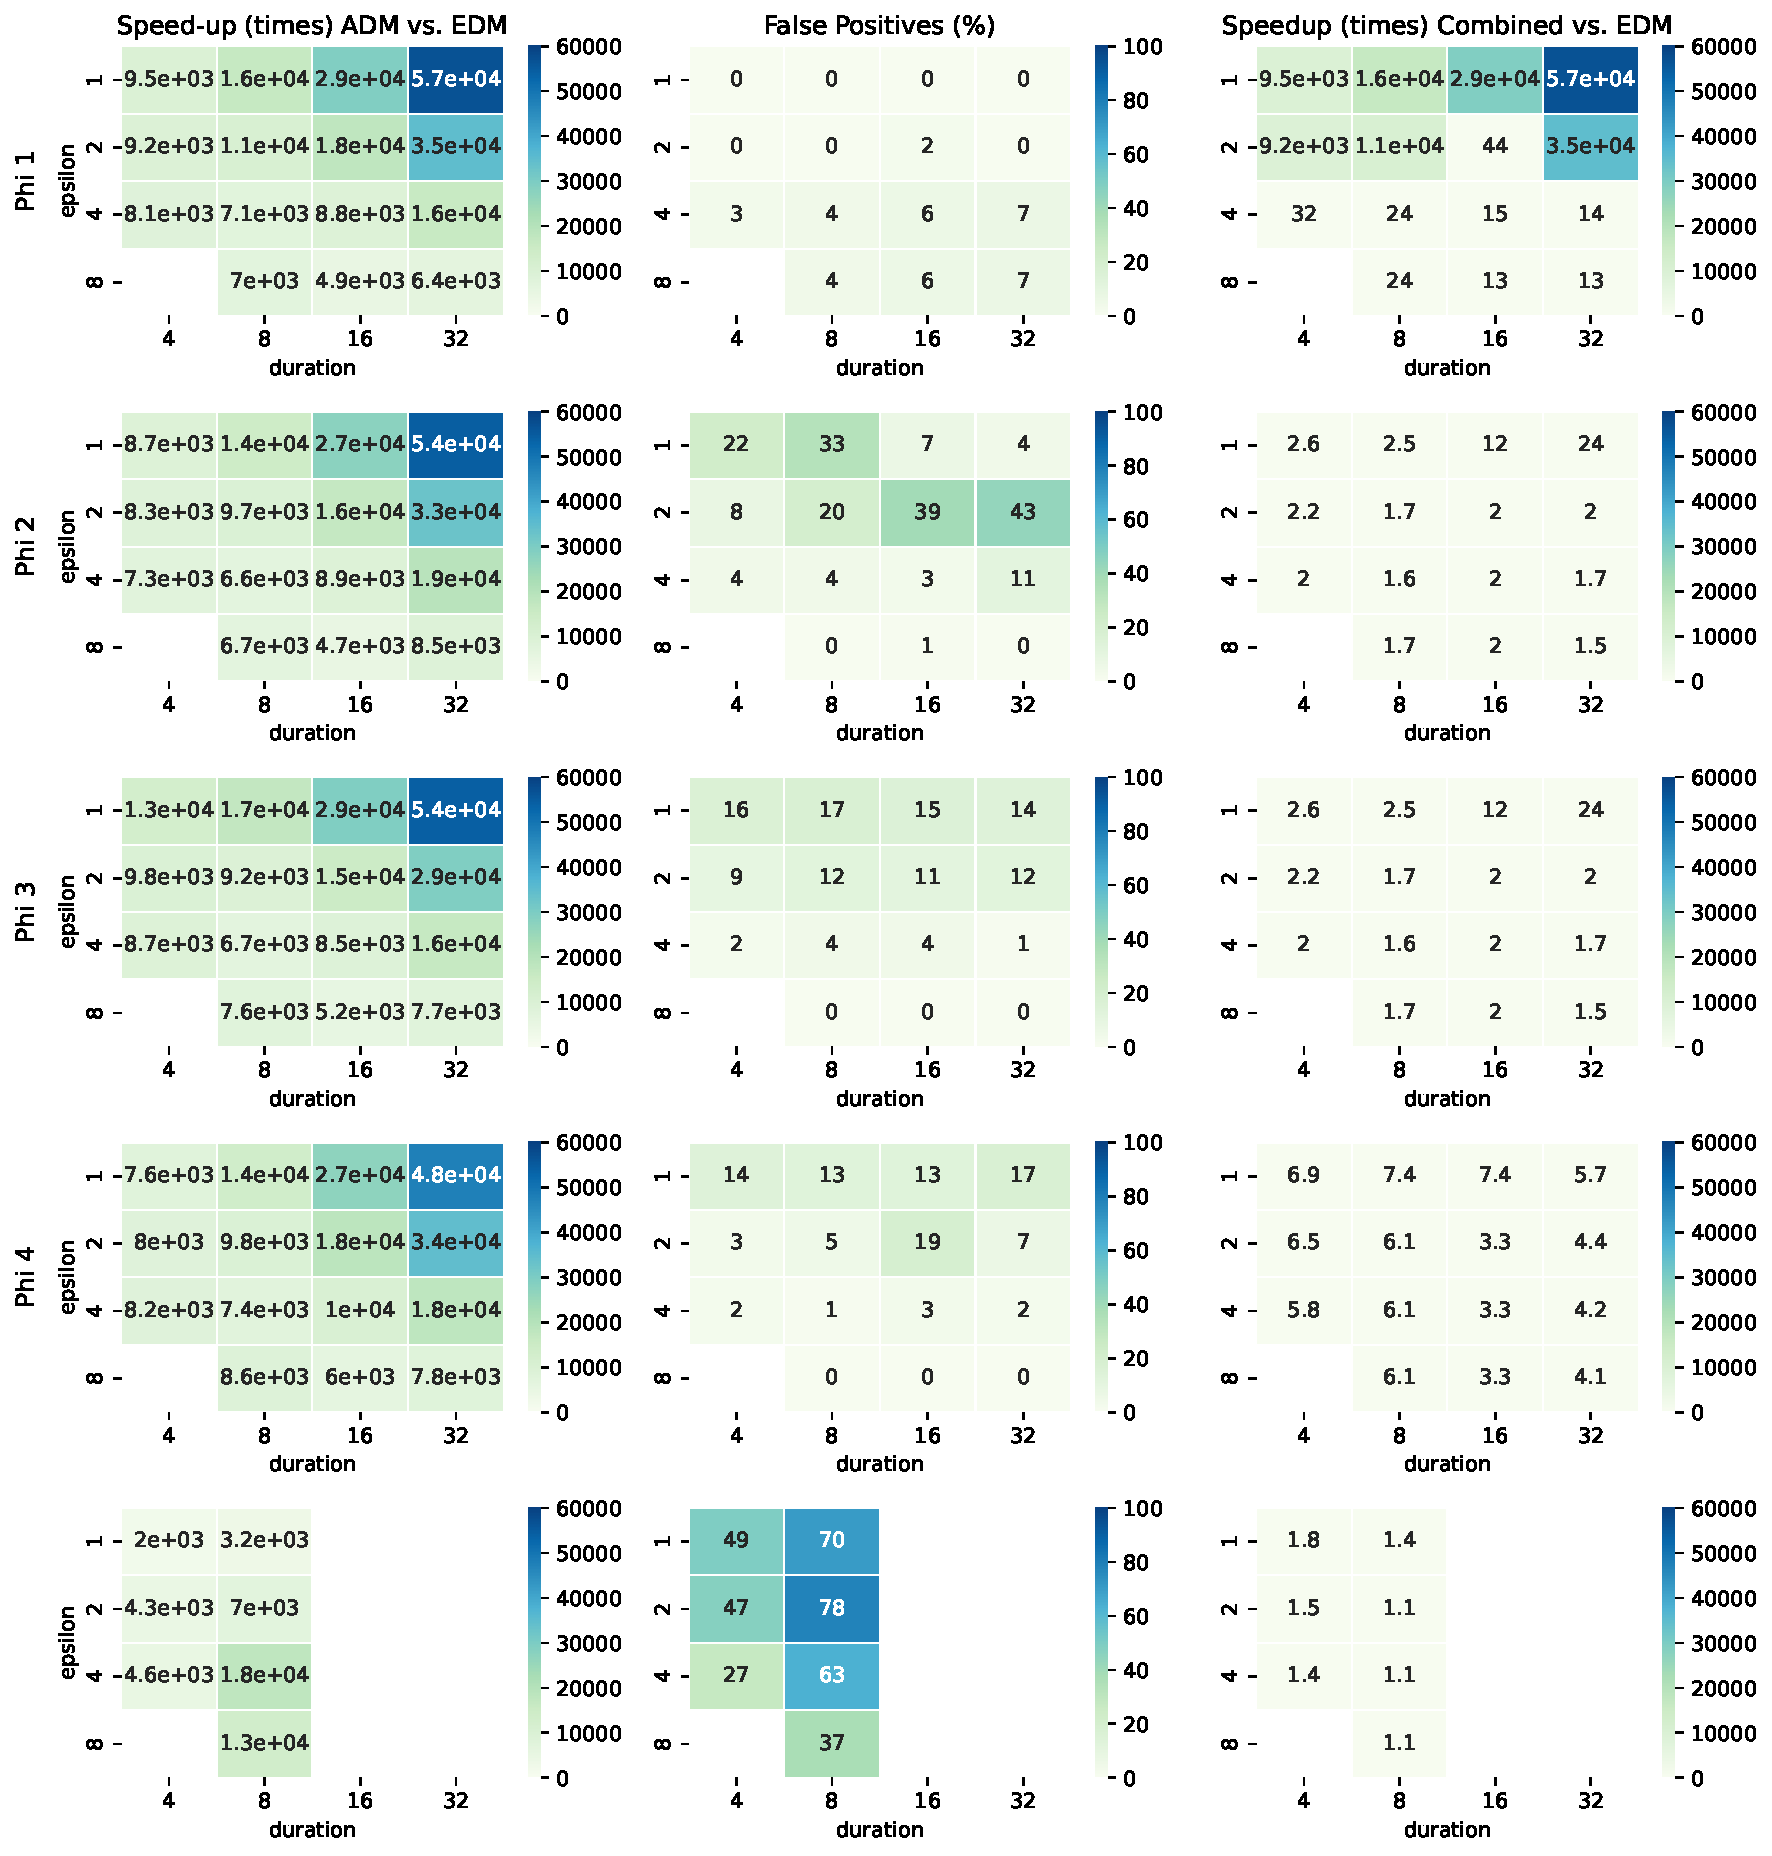
\includegraphics[width=\linewidth]{speedup}
\caption{The experimental results.}
\end{center}
\end{figure}